\setmainfont{Noto Serif}
\setsansfont{Noto Sans}
\setmonofont{Noto Sans Mono}
\setstretch{1.35}

\section{Электронная спектроскопия}
1. Студенту ФЕН НГУ вручили нитку из молекул полистирола и предложили построить такую геометрию эксперимента по исследованию анизотропии люминесценции, чтобы установить расположение бензольных колец в молекуле друг относительно друга. Каким образом необходимо провести данный эксперимент? Считать, что плоскости бензольных колец перпендикулярны направлению цепи, а цепь ориентирована строго вдоль нитки.\par
2С. Известны квантовые выходы и времена флуоресценции ($\phi_f^0$, $\tau_f^0$) и фосфоресценции ($\phi_p^0$, $\tau_p^0$) некоторого люминофора. Молекула Q тушит возбужденные синглетные и триплетные состояния люминофора с одинаковой константой скорости $k$. Получите выражение, аналогичное уравнению Штерна-Фольме-ра, для зависимости квантового выхода фосфоресценции $\phi_p$ от концентрации тушителя Q.
\par
\begin{wrapfigure}{r}{30mm} %this figure will be at the right
    \centering
    \vspace{-4.2ex}
    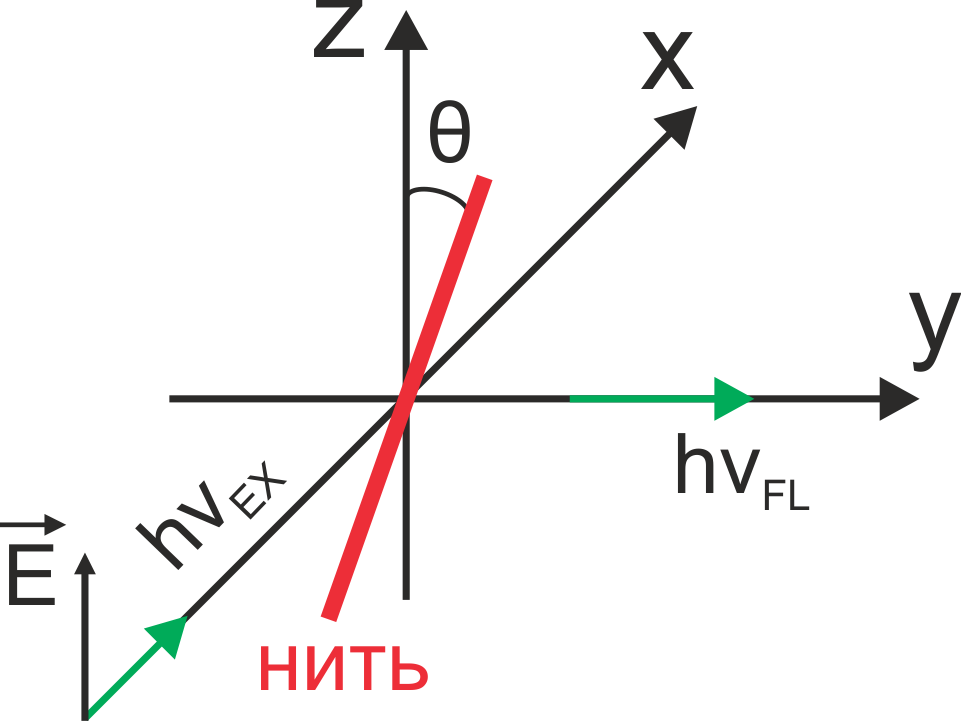
\includegraphics[width=28mm]{images/Fig_2_3_3.png}
    \vspace{-5ex}
\end{wrapfigure}
3С. Определить степень поляризации люминесценции для геометрии опыта, показанной на рисунке. Образцом является тонкая нить, в которой дипольные моменты всех молекул направлены вдоль оси нити. Нить лежит в плоскости $xz$ под углом $\theta$ к оси $z$.
\par
4К. Определите число разрешенных электрических дипольных переходов в молекуле аммиака. Между какими электронными состояниями они протекают?
\par
5С. Определите степень поляризации люминесценции при ее регистрации вдоль оси $x$ для твердого образца, в котором нет диффузии, если лазерное возбуждающее излучение распространяется по оси $y$, а электрическое поле лазерного излучения отклонено на угол $\theta$ от оси $z$.
\par
6К. Молекулярный кислород обладает значительной растворимостью во многих органических растворителях и воде, а также является тушителем люминесценции. Считая, что точность измерения времени жизни возбужденного состояния $\tau$ составляет 3\%, определите, начиная с какого $\tau$ растворенный кислород начинает оказывать влияние на экспериментально определенное время жизни возбужденного состояния некого люминофора в воде. Растворимость кислорода в воде равна 1,3$\cdot$10$^{-3}$ М, диффузионная константа скорости равна 10$^{10}$ М$^{-1}$$\cdot$с$^{-1}$.
\par
7Т. В какой из молекул (бензол, нафталин, антрацен) расщепление между уровнями $S_1$ и $T_1$ больше?
\par
8. Переход $S_0$ $\rightarrow$ $S_1$ в пиридине поляризован вдоль оси, перпендикулярной плоскости молекулы. Определить поляризацию перехода $S_0$ $\rightarrow$ $T_1$.
\par
9С. Каждая молекула донора D жестко связана с акцептором A так, что расстояние между ними равно $R_0$, где $R_0$ – радиус Ферстера. Время жизни возбужденного состояния D в отсутствии тушителя равно 1 мкс. В раствор добавлен еще один тушитель B с концентрацией 1 мМ. Определите константу бимолекулярного тушения донора D молекулой B, если квантовый выход люминесценции донора уменьшился в 3 раза по сравнению со случаем отсутствия обоих тушителей.
\par
10С. Определите степень поляризации люминесценции растянутой пленки, в~которой дипольные моменты люминесцирующих молекул могут находиться только в плоскости этой пленки. Возбуждающее лазерное излучение распространяется по оси $y$ и имеет $\sigma$ поляризацию, пленка расположена под углом $\phi$ к оси $z$, детектирование люминесценции происходит по оси $y$.
\par
11С. Квантовые выходы флуоресценции и фосфоресценции некоторого красителя равны по 0,5, а его время жизни флуоресценции составляет 10 нс. Определите константу скорости интеркомбинационной конверсии.
\par
12С. Определите степень поляризации люминесценции образца, в котором люминесцирующие молекулы находятся в жесткой молекулярной матрице, при его облучении двумя световыми потоками: (1) вдоль оси $z$ с поляризацией вдоль оси $y$, (2) вдоль оси $y$ с поляризацией вдоль оси $z$. Регистрация люминесценции производится вдоль оси $x$.
\par
\begin{wrapfigure}{r}{47mm} %this figure will be at the right
    \centering
    \vspace{0mm}
    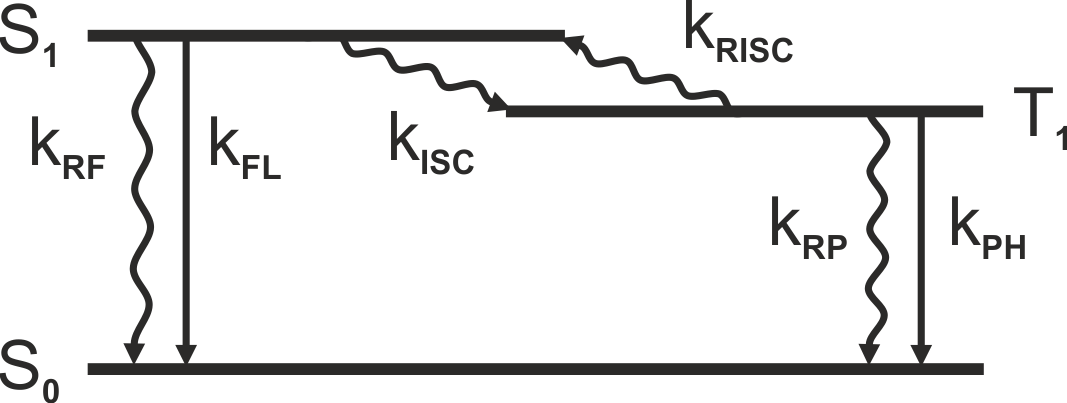
\includegraphics[width=47mm]{images/Fig_2_3_15.png}
    \vspace{-5mm}
\end{wrapfigure}
13К. Одним из способов повышения эффективности органических светодиодов является использование процесса термически активируемой задержанной флуоресценции (TADF). В простейшей трехуровневой TADF системе E-типа протекают процессы, изображенные на рисунке. Получите выражение для квантового выхода задержанной флуоресценции. Покажите, что его величина растет при увеличении $k_{RISC}$. Как вы считаете, с чем связано название процесса TADF?
\par
14К. Тушение кумарина C120 урацилом происходит по динамическому и статическому механизму. Определите динамическую константу тушения $k_q$ и~статическую константу равновесия $K_s$ реакции C120 + Q $\leftrightarrows$ [C120$-$Q], где Q – тушитель, если интенсивность флуоресценции падает в 1,26 раз при использовании 9,5~мМ концентрации тушителя. Время флуоресценции C120 без тушителя равно 5~нс. При концентрации тушителя 20 мM время флуоресценции укорачивается и~оказывается равным 3,85 нс.
\par
15Т. Относительный квантовый выход фосфоресценции нафталина при температуре 77 К зависит от концентрации бензофенона, выступающего в роли тушителя, в соответствии с таблицей, приведенной ниже. Выведите уравнение, описывающее $\phi/ \phi_0$ для данных экспериментальных условий, а также определите радиус тушения.

\begin{center}
\begin{tabular}{ c c c c c c c }

 $C$, M & 0 & 0,08 & 0,16 & 0,24 & 0,32 & 0,40 \\ 
 \hline
 $\phi / \phi_0$ & 1 & 0,65 & 0,45 & 0,23 & 0,19 & 0,13 \\  
\end{tabular}
\end{center}

\par
